\section{Project definitions manager}
\label{sec:project_definitions_manager}

\begin{figure}
    \centering
    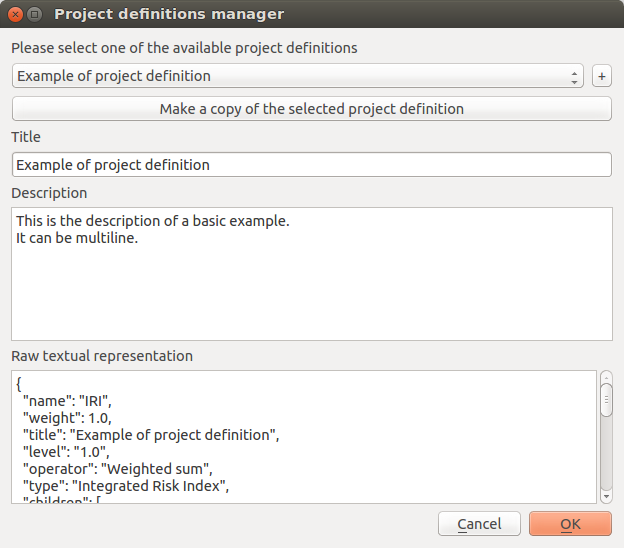
\includegraphics[width=\textwidth]{../images/image13}
    \caption{Project definitions manager}
    \label{fig:project_definitions_manager}
\end{figure}

The `Project Definitions Manager' is a module that was developed to allow users
to create multiple models that can be accessed with a click of a button using a
single layer. Each `project definition' (see Section~\ref{sec:definitions}) can
define a different model structure, weighting and aggregation scheme, and
variable selections among data available in the underlying layer. It allows
users to seamlessly toggle through various integrated risk assessment projects
without having to refer to different `QGIS projects' or different `layers'
containing data for a given area or areas, and without having to re-symbolize
data to compare results of assessments using different methodological
parameters. The `Project definitions manager' was developed around a dialog
window that enables users to edit the current project definition, to switch
from the current project definition to a different one, to add a new project
definition, or to clone an existing project definition.

While contributing to the `Title' and `Description' textbox of the project
definitions manager, the `Raw textual representation' is updated accordingly.
Please note that it is not recommended for users to edit the parameters
directly inside the `raw textual representation' portion of the project
definition manager, although it is not forbidden. This especially applies to
variable names (field names) and sub-indicators (also field names) defined by
nodes within the weighting and aggregation tree (see
Section~\ref{sec:weighting_and_calculating}). Manual adjustments can be useful
in some corner cases, by experienced users, but manual adjustments can cause
the toolkit to behave unexpectedly and can cause shapefiles to behave
unexpectedly. Users performing these adjustments are at risk of compromise
their data.

The `+' button at the right of the dropdown menu can be used to associate the
current layer with a new project definition. By clicking it, a new basic
project definition is created and the user is invited to provide the new
project definition with a title and, possibly, a description.  The button `Make
a copy of the selected project definition', assigns to the active layer within
the QGIS a new project definition that is an exact clone of the selected one.
Having two similar project definitions can be useful to easily visualize how
the output of a project is changed based on  updated variable selections,
weighting, and aggregation schemes. This visualization is possible because a
simple click is sufficient to switch between `before' and `after' project
definitions. When `OK' is pressed, the composite indices are re-calculated
accordingly with the project definition and the layer is styled as a
consequence via a default classification and symbolization that is adjustable
within the QGIS\@. This computation can take some time, depending on the
complexity of the layer.
